\chapter{Introduction}

\ifpdf
    \graphicspath{{Introduction/Figs/Raster/}{Introduction/Figs/PDF/}{Introduction/Figs/}}
\else
    \graphicspath{{Introduction/Figs/Vector/}{Introduction/Figs/}}
\fi

% References to check (FlexPointer)
% - [23, 25, 30, 57, 57, 58] -> Virtual memory infrstructure
In the dynamic landscape of computing, the pursuit of optimal performance is a constant endeavor, 
especially as applications evolve to handle increasingly complex workloads. 
One critical aspect influencing performance is memory management, where efficient 
utilization of resources is paramount. Translation Lookaside Buffers (TLBs) play a 
pivotal role in this regard, expediting memory access by storing recently accessed memory translations.
However, as applications grow in size and complexity, the capacity of TLBs often struggles to 
keep pace, leading to performance bottlenecks. To address this challenge, researchers have 
turned to innovative solutions, one of which involves harnessing the benefits of huge pages.
Huge pages, also known as large pages, allow for the allocation of memory in significantly 
larger chunks compared to traditional small pages. By reducing the number of TLB entries 
needed to access a given amount of memory, huge pages offer a potential avenue for optimizing 
TLB utilization and thereby enhancing overall system performance.

Simultaneously, advancements in hardware-level security, such as the Capability Hardware 
Enhanced RISC Instructions (CHERI) architecture, present additional opportunities for 
performance enhancement. CHERI's capability-based addressing approach not only strengthens 
system security by tightly controlling memory access but also provides avenues for 
accelerating memory management operations.

In this context, the integration of huge pages into memory management 
strategies alongside capability-based addressing in architectures like 
CHERI offers a compelling synergy. By optimizing TLB utilization through the 
utilization of huge pages and leveraging the security features of capability-based addressing, 
significant performance improvements can be realized. This approach not only enhances 
system security but also accelerates memory access. The following below are research questions 
we are addressing:
\begin{enumerate}
    \item Is there faster run times and lesser TLB misses when bounds are used not just for security but
    also to track memory allocations ? 
    \item Does using bounds to seek through physically contiguous memory reduce the complexity in standard 
    memory allocators that have features like transparent huge pages ?
  \end{enumerate}

% TODO: 
% - Add references for FlexPointer, Range Memory Mapping (RMM), Direct Segment and Huge Pages
\subsection{TLB based approaches}
Efficient memory management, particularly in the context of 
Translation Lookaside Buffer (TLB) optimization, has been a focal point of 
research and development within computer architecture. Various techniques have been 
proposed to mitigate TLB-related bottlenecks and improve overall system performance.

\subsubsection{Huge Pages:}
% This is used to map a very large region of memory to a 
% single entry. This small/large region of memory is physically
% contiguous. Most implementations of huge pages \cite{panwar_hawkeye_2019} are size
% aligned, For example for the x86 architecture the huge pages 
% size are 4KB, 2MB and 1GB pages. 
Increasing TLB reach can be achieved by using larger page sizes, such as huge pages, which are common in modern computer systems. 
The x86-64 architecture supports huge pages of 2 MB and 1 GB, backed by OS mechanisms like Transparent Huge Pages (THP) 
and HugeTLBFS in Linux. However, available page sizes in x86-64 are limited, leading to internal fragmentation issues. 
For instance, allocating 1 MB with 4 KB base pages requires 256 PTEs, but using a 2 MB huge page would waste 
half of the memory space. Some architectures offer more page size choices, such as Intel Itanium, which 
allows different areas of the address space to have their own page sizes. Itanium uses a hash page table to organize huge 
pages, but without significant changes to the conventional page table, it only helps reduce page walk overheads. 
HP Tunable Base Page Size permits the OS to adjust the base page size, but still faces internal fragmentation problems, 
with HP recommending a base page size of no more than 16 KB. Shadow Superpage introduces a new translation level 
in the memory controller to merge non-contiguous physical pages into a huge page in a shadow memory space, extending 
TLB coverage. However, this approach requires all memory traffic to be translated again in the memory controller, 
resulting in additional latency for memory accesses.
% \subsection{Tailored page sizes}
% TODO later
% \subsection{TLB coalescing}
% This leverages the default OS allocator behavior to pack
% multiple PTEs into a single TLB entry.

% Sources 
% - [14] Jonathan Corbet. 2009. Transparent Hugepages. (2009). Retrieved from https://lwn.net/Articles/359158/.
% - [15] Jonathan Corbet. 2011. Transparent huge pages in 2.6.38. (2011). Retrieved from https://lwn.net/Articles/423584/.

\subsubsection{Segment:}
% A segment\cite{basu_efficient_nodate} can be viewed as mapping between contiguous virtual
% memory and contiguous physical memory. The property of a 
% segment allows it to be larger than a page. Direct Segment allows the user to set a single segment
% for an application. Two registers are added to mark the start
% and end of the segment. Any virtual address within this region
% can be translated by adding the fixed offset between the virtual
% and physical address.
Early processors often used segments to manage virtual memory, where a segment essentially mapped contiguous 
virtual memory to contiguous physical memory. Unlike pages, which are relatively small, segments can be much 
larger, offering the potential for more efficient memory management in certain scenarios. 
This concept of segmentation has seen a resurgence in some modern approaches that aim to enhance 
translation coverage by designating specific areas in the virtual address space.
% Alternate segment technique
% - JayneelGandhi,ArkapravaBasu,MarkD.Hill,andMichaelM.Swift.2014.Efficientmemoryvirtualization:Reducing
dimensionality of nested page walks. In Proceedings of the MICRO’14. 178–189.
One such approach is Direct Segment. This method allows programmers to explicitly define 
a single segment for applications requiring significant memory. It introduces two new 
registers to the system, which indicate the start and end of this segment. 
Virtual addresses within this segment are translated by calculating 
the offset from the virtual start address and applying this offset to the 
physical start address. This straightforward method simplifies the translation 
process for large memory areas but requires significant modifications to the 
source code of applications.
% Do-it-yourself Virtual Memory
% - Hanna Alam, Tianhao Zhang, Mattan Erez, and Yoav Etsion. 2017. Do-It-Yourself virtual memory translation. In Pro- ceedings of the 44th Annual International Symposium on Computer Architecture (ISCA’17). Association for Computing Machinery, New York, NY, 457–468.
Another approach, Do-it-yourself Virtual Memory Translation (DVMT), similarly 
introduces two registers to define a special area within the virtual address space. 
However, DVMT supports more complex translation mechanisms. When an address 
within this designated area is accessed, DVMT initiates a dedicated 
thread to handle the translation. This flexibility allows for more 
sophisticated memory management techniques, but like Direct Segment, 
it necessitates extensive changes to the application's source code. 
Additionally, both Direct Segment and DVMT bypass the conventional page table 
for the special virtual area, operating independently of the standard 
paging mechanism.

\begin{figure}[h]
  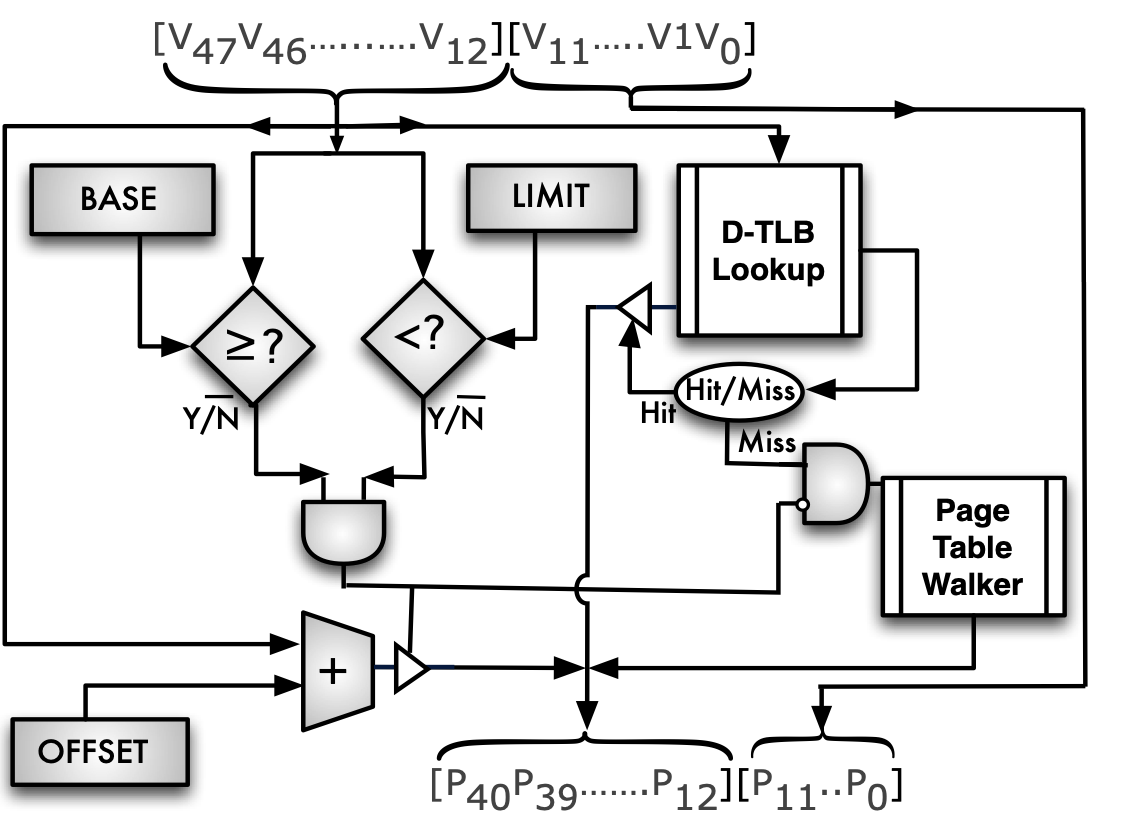
\includegraphics[width=0.9\textwidth]{segment.png}
  \caption{Logical view of address translation with direct segment\cite{basu_efficient_nodate}.}
  \label{fig:Segment}
\end{figure}

In Figure \ref{fig:Segment}, each data memory reference involves presenting the data virtual address 
V to both the new direct-segment hardware and the Data Translation Lookaside Buffer (D-TLB). If the virtual address 
V falls within the specified range defined by the direct segment's base and limit register values, the new hardware translates the address to a physical address by calculating 
V+OFFSET. This translation process bypasses the D-TLB, meaning that addresses handled by the direct-segment hardware do not experience TLB misses. 
It's important to note that the direct-segment hardware only allows read-write access.

\subsubsection{Range Memory Mapping (RMM):}
% RMM\cite{karakostas_redundant_2015} introduces the concept of adding an additional range table.
% For large allocations RMM eagerly allocates contiguous physical pages.
% The following allocations creates large memory ranges that are
% both virtually and physically contiguous. RMM builds on the concept
% of Direct segment by adding offset to translate a virtual address 
% to physical address. RMM compares address with range boundaries 
% to decide which range it belongs to. RMM queries the range table 
% ofter an L1 TLB miss.
Redundant Memory Mappings (RMM)\cite{karakostas_redundant_2015} enhance memory management by introducing an additional range table 
that pre-allocates contiguous physical pages for large memory allocations, creating ranges that 
are both virtually and physically contiguous. This approach simplifies address translation 
within these ranges by adding an offset, similar to Direct Segment, but RMM supports multiple 
ranges and operates transparently to programmers, requiring no source code modifications. 
The range table, separate from the conventional page table, holds the mappings for these 
large allocations. To determine which range an address belongs to, RMM compares the address 
against all range boundaries, a process that is computationally expensive and therefore performed 
only after an L1 TLB miss. To optimize this, RMM uses a range TLB (RTLB) to quickly identify 
if an address falls within any pre-allocated range, facilitating efficient translation and 
reducing overhead. Range mapping works alongside the paging system by generating TLB entries on 
TLB misses and still performing TLB lookups for each virtual address translation. 
Unlike traditional segmentation mechanisms, range mapping activates a range lookaside 
buffer (RTLB) located with the last level TLB upon a miss. The hardware TLB miss 
handler then searches the RTLB for the miss address and, if found, generates a new 
TLB entry with the physical address derived from the base virtual address and 
range offset, along with permission bits. If the RTLB also misses, the system 
defaults to a standard page walk while a range table walker simultaneously 
loads the range into the RTLB in the background, avoiding delays in memory operations. 
The RTLB, functioning as a fully associative search structure, ensures 
that most last level TLB misses are handled efficiently by range mapping, 
reducing the need for costly page table walks.

\begin{figure}[h]
  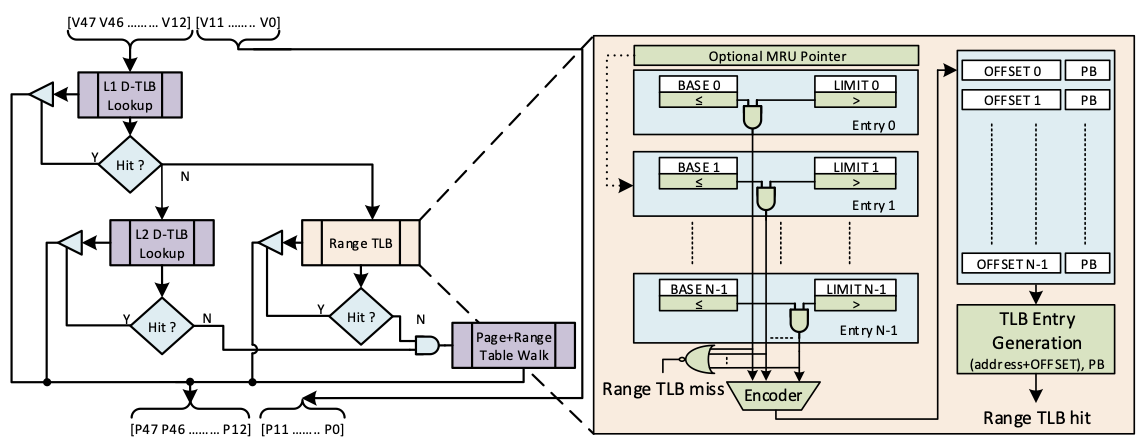
\includegraphics[width=0.8\textwidth]{rmm.png}
  \caption{RMM\cite{karakostas_redundant_2015} hardware support consists primarily of a range TLB that is accessed in parallel with the last-level page TLB.}
  \label{fig:RMM}
\end{figure}

In Figure \ref{fig:RMM} illustrates the structure and logic of the range TLB, which comprises N entries (e.g., 32). Each entry in 
the range TLB includes a virtual range and a corresponding translation. The virtual range contains the BASEi and LIMITi values, defining 
the boundaries of the virtual address range. The translation part holds the OFFSETi, which is the difference between the starting point 
of the range in physical memory and BASEi, as well as the protection bits (PB). Each range TLB entry is equipped with two comparators to facilitate lookup operations. 
When accessing the range TLB in parallel with the L2 TLB, after a miss at the L1 TLB, the hardware compares the virtual page number that missed in the L1 TLB against 
all ranges in the range TLB, checking if BASEi <= virtual page number < LIMITi. On a hit, the range TLB returns the OFFSETi and protection bits for the corresponding 
range translation, and calculates the corresponding page table entry for the L1 TLB. It does this by adding the requested virtual page number to the hit 
OFFSETi value to produce the physical page number, and copying the protection bits from the range translation. If there is a miss, the hardware fetches 
the corresponding range translation if it exists from the range table.



\subsubsection{FlexPointer:}
% FlexPointer\cite{chen_flexpointer_2023} is based on the RMM\cite{karakostas_redundant_2015} paper. FlexPointer
% does eagerly allocate pages which are physically contiguous and stores the ID to translate a virtual address 
% to physical address on the remaining unused bits on the 64 bit virtual address. 
% The paper contribution mentions shifting the TLB lookup to an earlier stage to improve
% latency of accessing the TLB entries. FlexPointer immediate queries the 
% range TLB for translations rather than the RMM paper which waits for the L1 TLB miss.
FlexPointer\cite{chen_flexpointer_2023} builds upon the range translation concepts found in RMM and Direct Segment. A range consists of contiguous virtual pages mapped 
to contiguous physical pages, with uniform protection bits, such as read, write, or execute. Defined by two addresses, BASE and LIMIT,
a range is base-page-aligned and can have an arbitrary number of pages. Due to the contiguous nature of these pages, 
all addresses within a range share a common DELTA, calculated as (physical\_address - virtual\_address). To translate a 
virtual address within a range, the processor simply adds DELTA to it.
\newline
A system employing range translations has three main components: 
(i) the creation of memory ranges, (ii) the management of range information, 
and (iii) the hardware that efficiently utilizes range translations. FlexPointer 
creates a range and assigns it a unique ID upon receiving a request for a large 
allocation. To ensure physical contiguity, it uses an eager paging strategy, 
which allocates physical pages at the time of the allocation request rather 
than on first access. This involves modifying memory management functions, 
such as malloc() and mmap(), to support eager allocation. Additionally, 
a kernel range table is used to record range translations, with mappings 
also maintained in the page table to ensure compatibility with other memory subsystems.
\newline
Similar to RMM, FlexPointer uses a range TLB to facilitate range translations in hardware. 
It can pass the range ID through the pointer tag, allowing the range TLB to operate in 
parallel with address generation. During a memory access, the processor uses the 
pointer tag to determine whether to search the range TLB or the page TLB, and the 
tag also guides which table to consult in the event of a TLB miss.

\begin{figure}[h]
  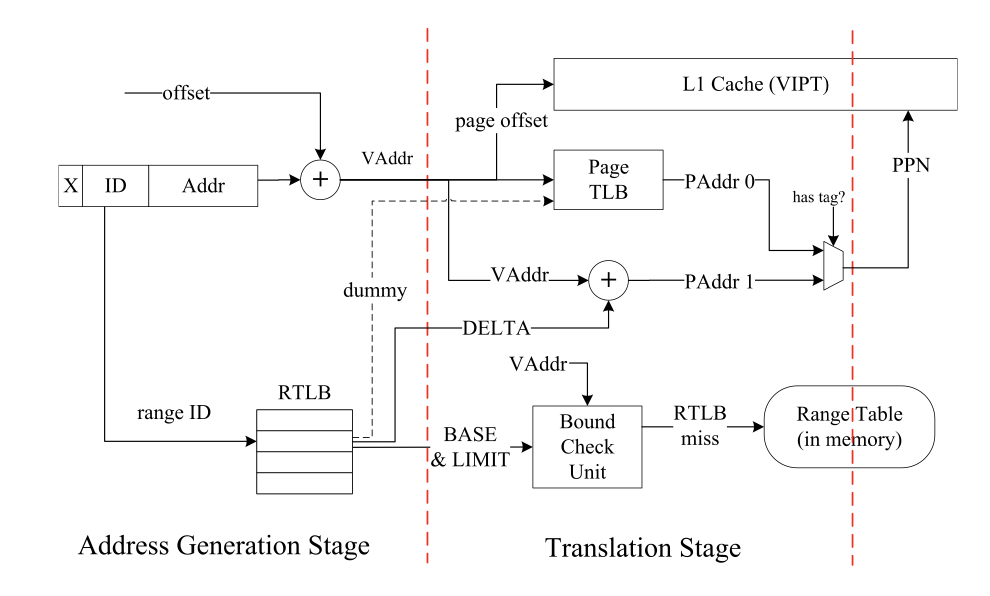
\includegraphics[width=0.8\textwidth]{flexpointer.png}
  \caption{FlexPointer\cite{chen_flexpointer_2023} hardware overview.}
  \label{fig:FlexPointer}
\end{figure}

% Illustrates the hardware components and workflow of FlexPointer. At the address generation stage, 
% the processor decides whether to query the range TLB or the page TLB according to the high bits
% of the address. If they are all 0s or 1s, then the address is translated with the original 
% page TLB after the address generation. Otherwise, the processor uses the range ID in the 
% pointer to search the range TLB at once. As we stated before, IDs are unique in the 
% range TLB, so the pro- cessor gets only one DELTA when the ID hits in the range TLB. 
% Next, the processor adds DELTA to the generated virtual address while comparing 
% the virtual address with BASE and LIMIT. If it passes the range check, then the 
% sum of DELTA and the virtual address is the correct physical address. Moreover, 
% if an address passes the boundary check of a dummy entry, it will be sent to 
% the page TLB for translation.

% A range TLB miss happens in two cases. (i) There is no matching ID in the range TLB. (ii) 
% The boundary check fails. When a range TLB miss happens, the processor handles it by starting 
% a range table walk to fetch the corresponding range translation. To simplify the range TLB lookup, 
% we want to keep IDs in the range TLB unique. So if the miss is caused by sub-range mismatching, 
% the newly fetched translation should be updated where the previous sub-range lies instead of 
% inserting a new entry. During a range table walk, we first calculate the translation entry 
% address by adding (ID << 5) to the base address of the range table (a range table entry 
% takes 32 bytes, as shown in Figure 4). The range table base address is part of the program 
% context and should be stored in a dedicated register, like storing the page table base in CR3. 
% If the address to be translated falls in [BASE, LIMIT ), then the entry is what we need and 
% will be fetched into the range TLB, whether it is a dummy entry or not. For a dummy entry, 
% we should query the page table for a correct translation and insert it into the page TLB. 
% When the address falls out of [BASE, LIMIT ), we check the L bit to see whether the current 
% entry is the last sub-range entry. If not, we get the next sub-range entry with NRID and 
% repeat the above procedure. But if it is the last one, then there must be a safety violation.

In Figure \ref{fig:FlexPointer} FlexPointer utilizes specialized hardware components and a streamlined workflow for efficient memory management. During address generation, 
the processor determines whether to query the range TLB or the page TLB based on the high-order bits of the address. 
If these bits are all 0s or 1s, indicating a regular page TLB operation, the address is translated accordingly 
post-generation. Alternatively, if the high bits suggest a range TLB operation, FlexPointer uses the range ID 
embedded in the pointer to directly access the range TLB. Each range ID in the TLB corresponds uniquely to a 
DELTA, simplifying translation. The processor adds this DELTA to the virtual address and performs a boundary check 
against the BASE and LIMIT of the range. If the address falls within this range, the sum of DELTA and the 
virtual address yields the correct physical address. Addresses failing the boundary check are directed to the 
page TLB for translation.
\newline
A range TLB miss occurs under two conditions: either no matching ID exists in the range TLB, or the 
address fails the boundary check of a dummy entry. In response to a range TLB miss, the processor 
initiates a range table walk to retrieve the corresponding range translation. To optimize TLB lookup 
efficiency, FlexPointer maintains unique IDs within the range TLB. If the miss results from a sub-range mismatch, 
the updated translation replaces the previous sub-range entry rather than adding a new one. During the 
range table walk, the processor computes the address of the translation entry by adding (ID << 5) to the base address of the 
range table. This base address, akin to storing the page table base in CR3, is part of the program context. If the address to be 
translated falls within the BASE and LIMIT range of the fetched entry, it is fetched into the range TLB, regardless of whether 
it is a dummy entry. For a dummy entry, the page table is queried for the correct translation, which is then inserted 
into the page TLB. If the address falls outside the (BASE, LIMIT) range and the entry is not the last sub-range (determined by the L bit), the processor 
retrieves the next sub-range entry with the NRID and repeats the process. However, if it is the last sub-range and a violation occurs, it 
indicates a safety breach.

\subsection{Capability machines}
% CheriOS (https://www.cl.cam.ac.uk/techreports/UCAM-CL-TR-961.pdf)
% A capability[39][89] is an unforgeable token that both names an object and confers the authority to the bearer 
% to act upon it. Capabilities can be delegated between principals to both identify an object, and simultaneously 
% grant some authority over it. Contrast this with other methods that use two channels to share objects, one for 
% the name, the other for authority. For example, on UNIX, a file name is transferred as a plain-string path, 
% and the authority to open it is transferred by separately modifying permissions. A capability-fied version would be a 
% 'path capability', which would not just represent a path but the authority to open it in specified modes.
% Every access to an object requires authorisation by a capability. It is impossible to confuse which authority 
% should be used for a particular operation as it forms part of the reference. The capability used is not always explicit. 
% Some machines, like the CAP, perform dynamic capability lookup. The CHERI[37] work defines the principle of intentional access as where, 
% if a set of authorities is available, the invoked authority is stated explicitly. Systems that are not explicit in which capability to use, 
% or eschew capabilities completely, are vulnerable to confused-deputy attacks. Capability systems that obey the principle (such as CHERI and CheriOS) are not.
% Capabilities also separate policy from enforcement, reducing complexity in parts of the system we must trust. Capabilities can be shared in a 
% decentralised way, determined by principals. As a result, capabilities tend to proliferate throughout a system. Revoking a capability is to
% globally destroy or invalidate it and potentially any capability derived from it. There is normally a trade-off in complexity of use, and 
% complexity of revocation. Some schemes[107] will use tracking structures that require upkeep, but facilitate revocation. CHERI requires no 
% such tracking, favouring a more complex revocation procedure to accelerate capability usage.
% Despite many notable examples,[78] most commercial systems today are not capability-based. 
% Modern filesystems, program permissions, and memory protection features all, for the most part, use ambient authority.
A capability is an unforgeable token that names an object and grants the bearer the authority to act upon it. Capabilities can be delegated between 
principals to both identify an object and grant authority over it, in contrast to other methods that use separate channels for 
naming and authority sharing. For instance, on UNIX, a file name is shared as a path, and the authority to open it is 
granted by adjusting permissions separately. In a capability system, a 'path capability' would not just represent a 
path but also the authority to open it in specific modes.
\newline
Every access to an object in a capability system requires authorization by a capability, making 
it clear which authority should be used for each operation as it is part of the reference. 
In some systems like the CAP architecture, dynamic capability lookup is performed. 
The CHERI work introduces the concept of intentional access, where the invoked authority 
is explicitly stated if a set of authorities is available. Systems that lack explicit 
identification of which capability to use or do not utilize capabilities at all are 
vulnerable to confused-deputy attacks, unlike capability systems that follow the 
intentional access principle, such as CHERI and CheriOS.
\newline
Capabilities also separate policy from enforcement, simplifying the parts of the 
system that need to be trusted. They can be shared in a decentralized manner 
based on principals, leading to a proliferation of capabilities throughout 
the system. Revoking a capability involves globally destroying or invalidating 
it and potentially any derived capabilities. The trade-off between the complexity 
of use and revocation exists in capability systems, with some schemes using 
tracking structures for revocation maintenance. CHERI, however, does not require 
such tracking and opts for a more intricate revocation process to enhance capability usage.
\newline

% Capability machines provide and enforce capabilities in hardware. This is advantageous 
% not just for performance, but also for reducing the trusted computing base. 
% Although currently unpopular, there have existed numerous capability machines, 
% both academically and industrially. The 1960s Burroughs B5000[88] stack machine 
% had a descriptor table for every program segment. An array access would first 
% calculate an index in the descriptor table and then indirect through it. 
% Descriptors had bounds, and hardware performed access checks. Although this 
% preceded the modern notion of a capability machine, the Burroughs B5000 was 
% the first to utilise tagged memory to distinguish between segment descriptors 
% (notionally capabilities) and other memory types. 
% This allowed entries to be loaded directly onto the stack.

Capability machines implement and enforce capabilities in hardware, 
offering benefits such as improved performance and a reduced trusted 
computing base. While currently not as popular, there have been many 
capability machines in academia and industry. One example is the \textit{Burroughs B5000} 
stack machine from the 1960s, which featured a descriptor table for each program segment. 
When accessing an array, an index in the descriptor table was calculated first, 
followed by an indirect operation through it. Descriptors in the table had bounds,
 and hardware was responsible for performing access checks. Although predating the 
 modern concept of a capability machine, the \textit{Burroughs B5000} was one of the first 
 to use tagged memory to differentiate segment descriptors (similar to capabilities) 
 from other memory types, enabling entries to be directly loaded onto the stack.
 \newline
 % The 1970 Cambridge CAP computer[96] was another early register-based capability machine. 
% The CAP computer used explicit capability registers, which it could load and store from 
% dedicated capability segments. Dedicated capability segments obviated tags, but prevented 
% mixing capabilities and data flexibly.

% Commercially, IBM's System/38,[61] and its successor the AS/400, were successes, and 
% like the B5000, featured tagged memory to distinguish capabilities from data. Intel's iAPX 432 
% was less successful due to poor performance, notably due to its poorly-optimised ADA compiler.[29] 
% It supported both hardware- and software-defined capabilities, differentiating between data 
% and capabilities like the CAP computer, by dividing segments.

% The M-Machine[50] used guarded pointers for capabilities, as described by Carter et al.[20] 
% It supported power-of-two sized bounds and bound alignments, using a fat pointer to encode bounds, 
% permissions, and an address. M-Machine capabilities supported two interesting capability variants: 
% a 'key' capability and an 'entry' capability. Neither could be modified or forged. Entry capabilities 
% could be jumped to, producing executable capabilities, and key capabilities served as identifiers. 
% A bit in executable capabilities encoded whether the processor was in supervisor mode. Combined 
% with entry capabilities, this allowed securely transitioning to privileged code at 
% pre-defined entry points using normal jumps.

% More recently, in 2013, LowFat[76] implemented hardware support for bounds checking fat pointers 
% compressed into 64 bits, with support for bounds-alignment not on a power-of-two. They are, 
% although similar to M-Machine and CHERI constructs, not capabilities. They lack authority, 
% unforgeability, and a facility for compartmentalisation.

The \textbf{1970 Cambridge CAP computer} was an early register-based capability machine that utilized explicit 
capability registers. These registers could be loaded and stored from dedicated capability 
segments, which did not require tags but limited the flexibility in mixing capabilities and data.
\newline
On the commercial front, \textbf{IBM's System/38} and its successor, the AS/400, were successful 
systems that, like the Burroughs B5000, incorporated tagged memory to distinguish 
capabilities from data. Intel's iAPX 432 faced challenges due to poor performance, 
particularly attributed to its inefficient ADA compiler. The architecture supported 
both hardware- and software-defined capabilities, dividing segments to differentiate 
between data and capabilities, similar to the CAP computer.
\newline
The \textbf{M-Machine} utilized guarded pointers for capabilities, with support for 
power-of-two bounds and alignments. A fat pointer encoded bounds, permissions, 
and an address for the capabilities. The M-Machine introduced two distinct 
capability variants: a 'key' capability and an 'entry' capability, both 
unmodifiable and non-forgeable. Entry capabilities could be executed, 
transforming into executable capabilities, while key capabilities 
functioned as identifiers. A supervisor mode bit in executable capabilities 
facilitated secure transitions to privileged code using normal jumps at predefined entry points.
\newline
In 2013, \textbf{LowFat} implemented hardware support for bounds checking fat pointers compressed into 
64 bits, with non-power-of-two alignment support. While similar to constructs seen in 
M-Machine and CHERI, these pointers lack some essential capabilities such as authority, 
unforgeability, and compartmentalization features.
\newline
% CHERI[136][135] was designed as part of the CTSRD project. It further refines hardware- enforced capabilities, 
% but with a goal shift to run existing MMU-based OSs, and mostly unmodified legacy C/C++ code. 
% Unlike M-Machine, CHERI avoids software-emulation for capability operations, 
% but still incorporates many of its ideas. 

CHERI, developed as part of the CTSRD project, enhances hardware-enforced capabilities 
with a focus on running existing MMU-based operating systems and mostly unchanged 
legacy C/C++ code. In contrast to the M-Machine, CHERI aims to avoid software 
emulation for capability operations while incorporating many of the M-Machine's concepts.

\subsubsection{Capability based operating systems}
Capabilities are beneficial not only for controlling access at the hardware level but also 
have applications in operating systems and software applications.
\newline
% An early system, Hydra,[137] was built atop the PDP-11. Hydra had capabilities for system- level objects and user-constructed objects. 
% All capability operations required syscalls as only the kernel could be trusted not to forge capabilities. This limited the frequency 
% of operations and which objects could practically be represented by capabilities. However, Hydra demonstrated implementation of the 
% object-capability model via IPC. 

The \textbf{Hydra system}, developed on the PDP-11, incorporated capabilities for both system-level 
and user-defined objects. Due to security concerns, all capability operations necessitated 
syscalls as only the kernel was deemed trustworthy to handle capabilities reliably. While 
this approach restricted the frequency of operations and the types of objects that 
could be effectively represented by capabilities, Hydra successfully showcased the 
practical implementation of the object-capability model through interprocess communication (IPC).
\newline
% KeyKOS (originally GNOSIS) was another early commercial capability OS, first developed for the IBM System/370, 
% and could support (among others) a UNIX environment.[60][17] KeyKOS, like most of the capability OSs discussed 
% here, was a message passing system, and used capabilities
% (which it called keys) to represent most system resources. KeyKOS separated the system 
% into domains, and gate keys could be invoked to send messages from one domain to another. KeyKOS implemented 
% a single-level persistent store. This store could be manipulated from userspace using capabilities, and was 
% transparently swapped with backing storage by the kernel. KeyKOS was followed by Eros,[118] and later Coyotos,[34] which 
% are both research focussed systems.

\textbf{KeyKOS}, originally known as GNOSIS, was an early commercial capability operating system designed 
for the IBM System/370 that could accommodate a UNIX environment. KeyKOS, similar to other 
capability-based operating systems mentioned, operated as a message-passing system and 
utilized capabilities termed as keys to represent various system resources. In KeyKOS, 
the system was divided into domains, with gate keys enabling message transfer between 
these domains. The OS featured a single-level persistent store that users could interact 
with using capabilities, and the kernel could seamlessly swap this store with backing storage. 
KeyKOS paved the way for subsequent research-oriented systems like Eros and Coyotos.
\newline
% The Mach microkernel[106][1] offered tasks, a collection of threads combined with a virtual address space. 
% The Mach abstraction for IPC was a port, which was much like a KeyKOS gate key. The authority to 
% communicate on a port was represented by a capability, and capabilities themselves could be 
% sent over ports for delegation. Messages, sent synchronously or asynchronously, were dynamically-sized 
% and typed. Like Hydra, Mach implemented an object-capability model using IPC. For example, creating 
% a thread required sending a message on a specific port, and the authority delegated by sending the port 
% capability. Mach aimed to provide a kernel compatible with a UNIX environment,[52] while hosting maximum 
% functionality outside of the kernel as a set of servers. Multiple UNIX variants have been derived from Mach, 
% or used Mach as a microkernel.

The \textbf{Mach microkernel} introduced the concept of tasks, which encompassed collections of threads 
combined with a virtual address space. In Mach, interprocess communication (IPC) was facilitated through 
ports, resembling KeyKOS gate keys, where the capability to communicate on a port was represented by a 
capability. Capabilities could be transmitted over ports for delegation, and messages, dynamically-sized 
and typed, could be sent synchronously or asynchronously. Similar to Hydra, Mach implemented an object-capability 
model using IPC, as exemplified by the process of creating a thread, which involved sending a message on a specific 
port and delegating authority by transmitting the port capability. Mach aimed to offer a kernel compatible with a 
UNIX environment while delegating maximum functionality outside of the kernel to a set of servers. Various 
UNIX variants have emerged from Mach or utilized Mach as a microkernel.
\newline
% The L4 microkernel was designed after Mach: its goal was to further reduce complexity and overheads compared with 
% past microkernels. It featured a simplified interface (an early version featured only 7 system calls[79]), offering 
% only threads, address spaces, and IPC. Simplified IPC meant that across-address-space message send on the first 
% L4 implementation was 20x[79] faster than Mach. SeL4,[72] is a formally-verified, from-scratch implementation of L4.
% SeL4 stores capabilities in a tree, where each node is an array of capabilities. Capabilities are fat-pointers to 
% objects in the physical memory space, begin untyped, and are re-typed to construct objects, such as page-tables. 
% Capabilities are only modifiable by the kernel, and are referenced from user-space via index.

Following the Mach microkernel, the \textbf{L4 microkernel} was developed with the aim of reducing complexity and 
overhead compared to previous microkernels. L4 featured a simplified interface, with an early version 
supporting only 7 system calls, providing functionality for threads, address spaces, and IPC. 
The streamlined IPC mechanism in L4 resulted in significantly faster across-address-space message transfers 
compared to Mach, with the initial L4 implementation being 20 times faster. SeL4, a formally-verified 
implementation of L4 built from scratch, stores capabilities in a tree structure where each node consists 
of an array of capabilities. Capabilities serve as fat-pointers to objects in physical memory, starting 
as untyped and then being retyped to create objects like page-tables. These capabilities can only be modified 
by the kernel and are accessed from user-space via an index.
\newline
% Barrelfish is an OS developed by ETH Zurich,[113] designed to better support large-scale heterogeneous systems. 
% Barrelfish uses capabilities[119] similar to seL4’s, with extensions to deal with the increased complexity of 
% deleting, copying, re-typing and revoking in a distributed fashion. Like other capability-based systems, 
% capabilities represent physical memory, kernel objects and communication end-points.

% Capsicum,[132] extends the POSIX API with file capabilities, and was prototyped on FreeBSD. Capability operations 
% still require system calls as FreeBSD runs on conventional hardware. Although files represent many things in UNIX, 
% Capsicum does not provide memory capabilities. Therefore, pointers shared between the OS and userspace can be arbitrarily fabricated.

% CheriBSD[37] augments FreeBSD to utilise CHERI hardware-enforced capabilities. CHERI capabilities can protect memory accesses 
% both in userspace compartments and the kernel. Being based on FreeBSD, much of the system interface is not capability based. 
% For example, spawning threads on FreeBSD is done via syscall, with ambient authority to do so. Mach would use a capability for 
% such an authority. While other capability OSs also have memory capabilities, their use is more coarse-grained than CheriBSD’s. 
% An OS like seL4 uses memory capabilities to, for example, grant the authority to create a page mapping. The use of that mapping, 
% via a load or store, will not check a capability. Also, because systems like seL4 use the MMU for enforcement, sizes and alignments of 
% objects capabilities refer to are necessarily quite coarse.

\textbf{Barrelfish} is an operating system developed by ETH Zurich specifically tailored to support large-scale heterogeneous systems. Utilizing capabilities 
similar to those in seL4, Barrelfish has extensions to manage the increased complexity of operations such as deletion, copying, re-typing, 
and revoking in a distributed manner. Capabilities in Barrelfish represent physical memory, kernel objects, and communication 
endpoints, adhering to the principles of capability-based systems.
\newline

\textbf{Capsicum} extends the POSIX API with file capabilities and was initially demonstrated on FreeBSD, where capability operations still require 
system calls due to the conventional hardware environment of FreeBSD. While files in UNIX systems can encompass various entities, 
Capsicum does not provide memory capabilities, allowing fabricated pointers to be exchanged between the operating system and user space.
\newline

\textbf{CheriBSD} enhances FreeBSD to utilize CHERI hardware-enforced capabilities for protecting memory accesses in both user space compartments 
and the kernel. Although CheriBSD operates on a FreeBSD base, many aspects of the system interface remain non-capability based. For instance, 
basic operations like spawning threads in FreeBSD require syscalls, granting ambient authority to do so, while Mach, in a capability-based system, 
would utilize a capability for such privileges. In comparison to other capability-based operating systems, CheriBSD's use of memory capabilities 
is more fine-grained, enabling precise control over memory accesses and operations. Systems like seL4 use memory capabilities for defining privileges 
like creating page mappings, although the actual use of these mappings during load or store operations may not involve capability checks. Additionally, 
since enforcement in systems like seL4 relies on the MMU, capabilities in these systems may refer to objects with coarse sizes and alignments.

\subsection{CHERI}
% source: https://www.cl.cam.ac.uk/techreports/UCAM-CL-TR-984.pdf
% Capability Hardware Enhanced RISC Instructions (CHERI) extends existing ISAs with hardware-defined 
% capabilities. CHERI aids adoption by being backwards compatible with existing software. 
% The most mature instantiation of CHERI is currently CHERI-MIPS, having both a simulator 
% and FGPA implementation. Disambiguating CHERI and CHERI-MIPS is unimportant for the 
% purposes of this document, apart from noting that although CheriOS was developed atop 
% CHERI-MIPS, it is unreliant on MIPS-specific features. Both CHERI-RISCV and CHERI-ARM
% (codenamed Morello[92][55]) are under development.

% CHERI is an instruction set extension, changing an existing ISA by requiring memory accesses to be performed through tagged capabilities, and adding 
% instructions for inspecting and manipulating capabilities [136]. Starting as an extension to the MIPS ISA [136, 137], CHERI has seen increasing 
% interest throughout this project, for example in Arm’s Morello experimental prototype, adding CHERI to a commercial Arm processor [54].

CHERI is an instruction set extension that modifies an existing ISA by mandating memory accesses to be conducted via tagged 
capabilities and introduces instructions for examining and modifying these capabilities. Initially developed as an 
enhancement to the MIPS ISA, CHERI has gained significant traction within the technology community, 
with notable implementations such as the Arm's Morello experimental prototype integrating CHERI into a 
commercial Arm processor.
\newline
% CHERI protects the integrity of pointers with a one-bit out-of-band tag. The hardware guarantees that every tagged capability must have been derived 
% from an initial root capability by a sequence of permissible operations, each of which can only monotonically decrease the rights granted by that capability. 
% This ensures all tagged capabilities have strict provenance. The tags prevent corruption of pointers, immediately mitigating a large class of attacks that 
% require manipulating pointers by overwriting them with non-capability data, for example Return-Oriented Programming [108]. In turn, by requiring every memory 
% access to quote a tagged capability, this protects data from accidental or malicious corruption, since the capability contains the intended bounds and permissions. 
% This too immediately mitigates some of the most common attacks, most notably buffer overflows [77].
% A study by Microsoft revealed that roughly 75\% of their security bugs are bounds overflows or temporal safety issues, indicating they would be mitigated by CHERI with 
% temporal safety support [65]. This provides assurance that CHERI can have a real impact on industry and users. In addition, monotonicity of the ISA has been formally proven, 
% showing that the intended invariants are provided by the architecture, if implemented correctly [15].

CHERI enhances pointer protection by incorporating a one-bit out-of-band tag to ensure the integrity of pointers. Each tagged capability in CHERI is required to originate from an initial root capability through a series of permissible 
operations, with each operation reducing the granted rights in a strictly decreasing manner. This strict provenance of tagged capabilities minimizes the 
risk of pointer corruption and effectively counters attacks that 
involve manipulating pointers by substituting them with non-capability data, such as Return-Oriented Programming.
\newline
The tags associated with capabilities in CHERI prevent pointer corruption and bolster security by necessitating that every memory access is 
associated with a quoted tagged capability that encompasses the intended boundaries and permissions. This measure serves to safeguard data 
from both accidental and malicious tampering, effectively mitigating common attacks like buffer overflows. A report by Microsoft highlighted that 
approximately 75\% of their security vulnerabilities are related to bounds overflows or temporal safety issues, indicating that CHERI's support for temporal safety 
could significantly address such issues and provide substantial benefits to the industry and users.
\newline
Furthermore, the monotonicity of the CHERI ISA has been formally verified, demonstrating that the architecture, if correctly implemented, upholds the 
intended invariants, offering a high level of security assurance.
\newline
\textit{The bit pattern of a capability consists of:}
\begin{itemize}

\item \textbf{Capability tag:} A one-bit out-of-band field that records whether the capability is valid, i.e. whether it has been derived only 
via legal monotonic operations.

\item \textbf{Cursor:} A field giving the current address referred to by the capability. This is all 
that is present in a traditional C pointer and the natural integer interpretation of the capability.

\item \textbf{Bounds information:} The capability only grants access to a single contiguous region of memory, specified by the bounds field. Changes to the capability can only ever grant access 
to a subset of the bounds without triggering an exception or clearing the tag.

\item \textbf{Permissions:} Permissions are required to access memory in different ways: most obviously read, write, and execute, but also the permissions to read and write capabilities, and more
experimental uses. These can only be modified by a bitwise AND operation, inherently guaranteeing monotonicity.

\item \textbf{Object type (otype):} CHERI provides a compartmentalisation mechanism for granting protected access to objects, represented as a 
pair of code and data. Code and data can be sealed with an otype, and primarily only unsealed by the CInvoke instruction, which atomically jumps to the code pointer and installs 
the unsealed data capability. Sealed capabilities cannot be mutated other than via a legal CInvoke or CUnseal instruction without 
raising an exception or clearing the tag.

\end{itemize}

\begin{figure}[h]
  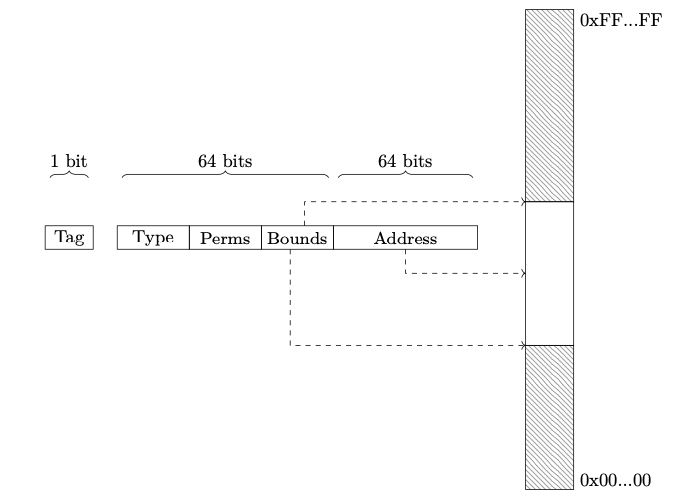
\includegraphics[width=0.8\textwidth]{chericapability.png}
  \caption{CHERI capability.}
  \label{fig:FlexPointer}
\end{figure}

\subsubsection{CHERI compression}
% One of the major performance overheads of CHERI comes from the increased widths of capabilities compared to 
% traditional pointers. This uses hardware resources, as the register file is bigger, but also adds cache pressure, as pointers 
% in memory must be accompanied by metadata. These effects can be somewhat mitigated by capability compression [135], which 
% reduces the bounds metadata to as little as 39 bits for a 64-bit pointer at the expense of alignment constraints on 
% representable positions for large objects. The compression and decompression is performed directly by the hardware, 
% allowing software to be largely unaffected.

% Capability compression, described in detail in our CHERI-Concentrate paper [135], stores the bounds as a base (B) of b bits, a top (T) of (b−2) bits, 
% and an exponent (E) of e bits. The described bounds are relative to the cursor of the capability (C). The actual base is determined by shifting B left by E, 
% filling any remaining upper bits with the corresponding most significant bits of C. The top is similar, except the top two bits of T are determined in the 
% common case by adding 1 to those of B. As a result, bounds are zero-filled in the least significant E bits, imposing the requirements on bound-alignment 
% mentioned above. To save some space, E is only stored when non-zero, in which case (called the internal exponent case) it takes the place of the least 
% significant bits of B and T (which are then implicitly zero). This means smaller objects can be represented more precisely than larger ones. The scheme 
% is currently implemented with b = 14, e = 6 for a 64-bit address space and b = 8, e = 6 for a 32-bit address space.

% Bounds with insufficient alignment to be represented as above are said to be unrepresentable. 
% CHERI offers two variants of the CSetBounds instruction: one triggers an exception when 
% unrepresentable bounds are requested, the other just returns the closest larger 
% representable bounds. In order to guarantee spatial safety, software must add padding 
% (at most 0.2\% or 12.5\% of the size of the object for 64-bit and 32-bit address spaces respectively) 
% at the beginning or end of large objects to ensure no other objects use the memory that is within the 
% bounds due to the rounding. Instructions that modify a capability cursor may also change the 
% interpretation of the bounds if they modify bits of the cursor that are used to determine the 
% base and top. Care is taken in the ISA and implementations that such cases clear the tag of the resulting 
% capability or raise an exception.

One of the significant performance challenges of CHERI stems from the larger size of capabilities compared to traditional pointers, leading to 
increased hardware resource usage and cache pressure. 
An approach to mitigate this impact is capability compression, as outlined in the CHERI-Concentrate paper. This method reduces bounds metadata 
to as few as 39 bits for a 64-bit pointer, albeit with alignment constraints on representable positions for larger objects. Hardware handles 
compression and decompression, ensuring minimal software impact.

In capability compression, bounds consist of a base (B) with b bits, a top (T) bits, and 
an exponent (E) with e bits relative to the cursor of the capability (C). The base is calculated by shifting B 
left by E and filling remaining upper bits with the corresponding most significant bits of C. The top follows a 
similar process, with the top two bits of T determined by adding 1 to those of B in the standard case. Bounds 
are zero-filled in the least significant E bits, enforcing bound-alignment requirements. The internal exponent case stores E only 
when non-zero, serving as the least significant bits of B and T, thereby allowing more precise representation of smaller objects.

The CSetBounds instruction in CHERI offers two variations: one triggers an exception for unrepresentable bounds, while the other returns 
the closest larger representable bounds. To ensure spatial safety, software must include padding (up to 0.2\% or 12.5\% of the object size 
for 64-bit and 32-bit address spaces, respectively) at the beginning or end of large objects to prevent memory usage conflicts resulting 
from rounding. Instructions altering a capability cursor may impact bounds interpretation if they modify cursor bits determining the 
base and top. Careful design in the ISA and implementations ensures these cases clear the capability tag or raise exceptions where necessary.













% \subsection{CHERI}
% A capability functions as a token that provides the holder with the authority to 
% execute specific actions. By carefully managing who possesses these capabilities, 
% it is possible to enforce security measures, such as ensuring that a particular
% section of software can only read from a designated range of memory addresses.

% The concept of cap  abilities has a rich history in computer science, tracing 
% back to early systems designed to enhance security and manage resources effectively.
% For instance, foundational work discussed in sources like \cite{noauthor_capability-based_nodate} offers a comprehensive 
% narrative on the evolution of capability architectures. This historical perspective 
% can be further enriched by incorporating insights from more recent studies, 
% such as those found in \cite{miller_towards_nodate}.

% CHERI (Capability Hardware Enhanced RISC Instructions)\cite{woodruff_cheri_2019} represents a modern embodiment of this 
% long-standing idea. It introduces more granular control over permissions, allowing for finer 
% distinctions in what actions can be performed and by whom. Moreover, CHERI is designed to integrate 
% seamlessly with contemporary processor instruction sets, ensuring that these advanced security 
% features can be implemented on modern hardware platforms. This adaptation not only revitalizes 
% the capability concept but also significantly enhances its applicability and effectiveness 
% in current computing environments.